\section{Quantum-classical correspondence and time reversal}
\label{sec:correspondence}

The two theories follow each other closely for a short time and statistically for longer, and then part
ways for good. A time-reversal experiment shows the deeper difference behind this (experiment 06,
\cref{fig:time_reversal}). We run $n$ kicks forward, then $n$ kicks backward with the exact inverse map or the
exact inverse Floquet step, and measure how far the result is from the starting point. Without roundoff both
would return exactly.

\begin{figure}[!tbp]
  \centering
  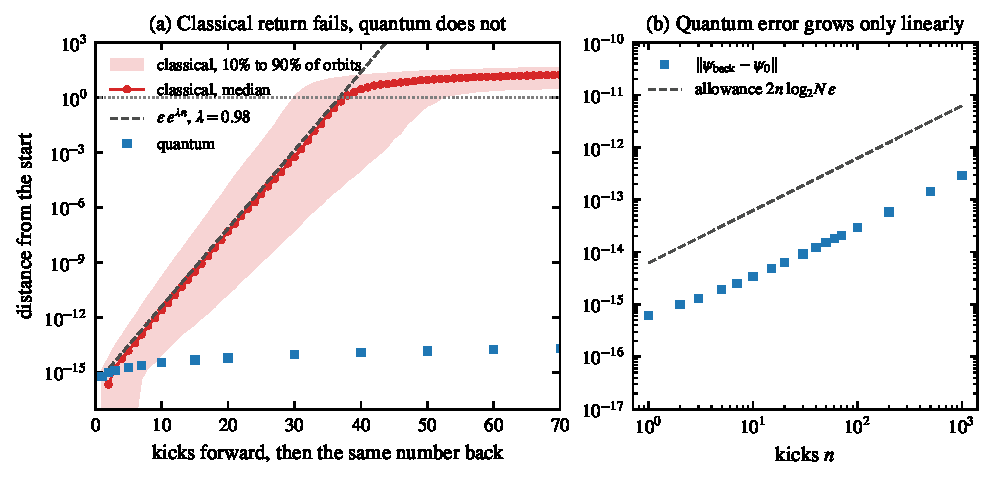
\includegraphics[width=\linewidth]{06_time_reversal.pdf}
  \caption{Time reversal at $K = 5$ (experiment 06). (a) Distance from the starting point after $n$ kicks
  forward and $n$ back. Red: median over 4000 classical orbits ($p_0 = 0$, $\theta_0$ uniform), with the band
  from the 10th to the 90th percentile; dashed: $\varepsilon\,\ee^{\lambda n}$ with the measured
  $\lambda = 0.98$. Blue: the quantum state ($\hbar = 0.25$, $N = 2^{14}$). (b) The quantum error up to 1000
  kicks, against the roundoff allowance $2n\log_2 N\,\varepsilon$.}
  \label{fig:time_reversal}
\end{figure}

For the classical orbits each step rounds the result to about $\varepsilon = 2.2\times10^{-16}$, and chaos
stretches such an error by about $\ee^{\lambda}$ per kick. The median return distance indeed grows like
$1.5\times10^{-16}\,\ee^{0.972n}$, close to the measured $\lambda = 0.981$ of the same orbits, and it first
exceeds 1 at $n = 38$, against the prediction $\ln(1/\varepsilon)/\lambda = 36.7$. After that the
``reversed'' orbits are as far from their starting points as random points on the chaotic sea. The quantum
state, on the other hand, returns to within $3.4\times10^{-15}$ after 10 kicks forward and back,
$3.0\times10^{-14}$ after 100 and $2.9\times10^{-13}$ after 1000. The error grows only linearly, at about a
twentieth of the roundoff allowance.

The reason is that the Schr\"odinger equation is linear and its evolution unitary. If $\delta$ is the error
made at some step, then $\|\hat U(\psi + \delta) - \hat U\psi\| = \|\delta\|$: later steps carry the error
along without magnifying it, and the errors from different steps at most add up. Exponential sensitivity in
the sense of classical chaos is impossible for a wave function. It is worth noting that the classical
Liouville equation for a phase-space density is also linear and conserves the density's norm. What amplifies
roundoff is following individual trajectories, not classical mechanics as such.

We also saw this effect without intending to. The same code run on a Windows laptop and on a Linux server
gave every quantum number to all printed digits, but every classical number came out slightly different: for
example $D = 12.44 \pm 0.10$ on one and $12.51 \pm 0.10$ on the other. The only operation in the standard
map that IEEE floating-point arithmetic does not fix exactly is the sine, which the two NumPy builds can
round differently in the last bit. Chaos amplifies that difference until, after about 37 kicks at $K = 5$,
every orbit is different, and ensemble averages then agree only within their statistical errors (which we
checked: 32 independent ensembles of 40000 orbits scatter by 0.103 around the mean $D$, against a stated
error of 0.099). At $K = 22$, where $\lambda \approx \ln 11 \approx 2.4$, the two machines' correlation sums
of \cref{fig:diffusion}(c) agree through lag 8 and differ by lag 16: roundoff needs only about 15 kicks to
grow to order 1 there.

Putting this together, there are three time scales. Up to the Ehrenfest time
$t_E \sim \lambda^{-1}\ln(1/\hbar)$, a few kicks, quantum expectation values follow the classical ones in
detail. Up to the break time $t^* \sim D/\hbar^2$, they follow them only statistically: the energy grows at
the classical diffusion rate even though individual quantities differ. After $t^*$ the discreteness of the
quasienergy spectrum takes over and the growth stops. For $\hbar = 0.25$, $t_E$ is about one kick, the 25\%
criterion puts the break at 20 kicks, and the saturation is complete after a few hundred kicks, of the order
of $\xi = 200$. The classical limit is recovered as $\hbar\to0$ at fixed $n$, because both $t_E$ and $t^*$ go to
infinity, but at any fixed $\hbar$ the long-time behavior is fundamentally quantum.
